\documentclass[crop=false]{standalone}
%\documentclass{standalone}
\usepackage{tikz} % To generate the plot from csv
\usepackage{pgfplots}
\usepackage{graphicx}
\usepackage{booktabs}
\usepackage{subfig}
\usepackage{float}
\usepackage[section]{placeins} % getting figures below sections
\usepackage{blindtext}
\usepackage{siunitx}
\usepgfplotslibrary{units} % Allows to enter the units nicely
\usetikzlibrary{external} %https://tex.stackexchange.com/questions/1460/script-to-automate-externalizing-tikz-graphics
\tikzexternalize[prefix=savedfigures/]

\pgfplotsset{compat=newest} % Allows to place the legend below plot
\usepackage{pgfplotstable}
\usepgfplotslibrary{statistics}

% #################### Function definition for box plots read table ##################\
\makeatletter
\pgfplotsset{
	boxplot prepared from table/.code={
		\def\tikz@plot@handler{\pgfplotsplothandlerboxplotprepared}%
		\pgfplotsset{
			/pgfplots/boxplot prepared from table/.cd,
			#1,
		}
	},
	/pgfplots/boxplot prepared from table/.cd,
	table/.code={\pgfplotstablecopy{#1}\to\boxplot@datatable},
	row/.initial=0,
	make style readable from table/.style={
		#1/.code={
			\pgfplotstablegetelem{\pgfkeysvalueof{/pgfplots/boxplot prepared from table/row}}{##1}\of\boxplot@datatable
			\pgfplotsset{boxplot/#1/.expand once={\pgfplotsretval}}
		}
	},
	make style readable from table=lower whisker,
	make style readable from table=upper whisker,
	make style readable from table=lower quartile,
	make style readable from table=upper quartile,
	make style readable from table=median,
	make style readable from table=average,
	make style readable from table=lower notch,
	make style readable from table=upper notch
}
\makeatother
\begin{document}

\section{23 3 Mumford1 SA Mutations AMALGAM 20210815 221210}

% ######################## UTRP SA Mutation operators applied ######################## 
\begin{figure} 
\centering 
\tikzsetnextfilename{UTRP_DBMOSA_BP_mutation_funcs_Best_comp} 
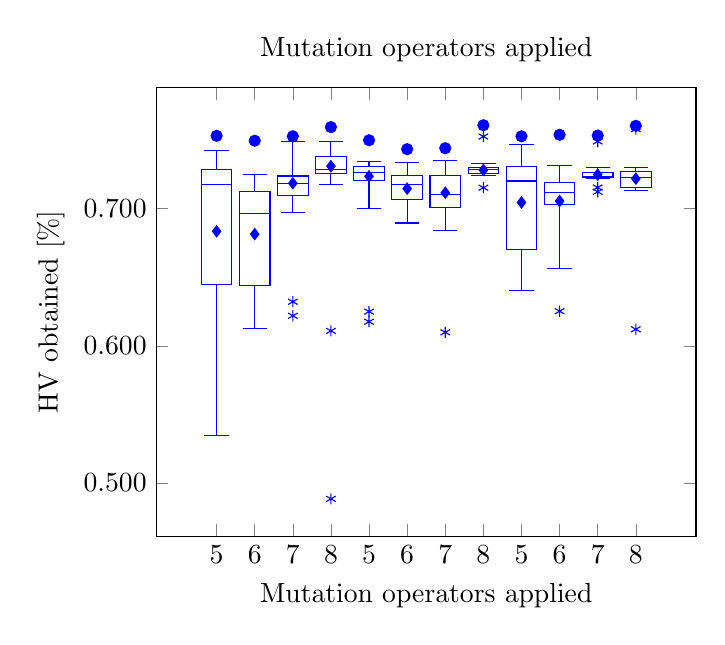
\begin{tikzpicture} 
\begin{axis}[ 
title={Mutation operators applied}, 
boxplot/draw direction=y, 
xtick={1,2,3,4,5,6,7,8,9,10,11,12}, 
xticklabels={5,6,7,8,5,6,7,8,5,6,7,8}, 
x tick label style={rotate=0, align=center}, 
xlabel={Mutation operators applied}, 
y tick label style={/pgf/number format/.cd,fixed,precision=3, zerofill}, 
ylabel={HV obtained [\%]}, 
] 

% ############## B_Mutations_AMALGAM=5 ################## 
\addplot[boxplot, mark=asterisk, 
boxplot prepared={ 
lower whisker=0.53483, 
upper whisker=0.74254, 
lower quartile=0.64475, 
upper quartile=0.72887, 
median=0.71785, 
average=0.68359}, 
color = blue, solid, area legend] 
coordinates {}; 
\addplot[only marks,mark=*,color = blue]coordinates{(1,0.75319)}; 

% ############## B_Mutations_AMALGAM=6 ################## 
\addplot[boxplot, mark=asterisk, 
boxplot prepared={ 
lower whisker=0.61292, 
upper whisker=0.72511, 
lower quartile=0.64405, 
upper quartile=0.71264, 
median=0.6963, 
average=0.68149}, 
color = blue, solid, area legend] 
coordinates {}; 
\addplot[only marks,mark=*,color = blue]coordinates{(2,0.74963)}; 

% ############## B_Mutations_AMALGAM=7 ################## 
\addplot[boxplot, mark=asterisk, 
boxplot prepared={ 
lower whisker=0.69714, 
upper whisker=0.74889, 
lower quartile=0.70972, 
upper quartile=0.72389, 
median=0.71871, 
average=0.71859}, 
color = blue, solid, area legend] 
coordinates {
(3,0.62196)
(3,0.63217)}; 
\addplot[only marks,mark=*,color = blue]coordinates{(3,0.75286)}; 

% ############## B_Mutations_AMALGAM=8 ################## 
\addplot[boxplot, mark=asterisk, 
boxplot prepared={ 
lower whisker=0.71749, 
upper whisker=0.74937, 
lower quartile=0.72603, 
upper quartile=0.73795, 
median=0.7284, 
average=0.73109}, 
color = blue, solid, area legend] 
coordinates {
(4,0.61093)
(4,0.48844)}; 
\addplot[only marks,mark=*,color = blue]coordinates{(4,0.75956)}; 

% ############## B_Mutations_AMALGAM_every_n=5 ################## 
\addplot[boxplot, mark=asterisk, 
boxplot prepared={ 
lower whisker=0.7005, 
upper whisker=0.73416, 
lower quartile=0.72081, 
upper quartile=0.73074, 
median=0.72638, 
average=0.72367}, 
color = blue, solid, area legend] 
coordinates {
(5,0.62499)
(5,0.61763)}; 
\addplot[only marks,mark=*,color = blue]coordinates{(5,0.74998)}; 

% ############## B_Mutations_AMALGAM_every_n=6 ################## 
\addplot[boxplot, mark=asterisk, 
boxplot prepared={ 
lower whisker=0.6896, 
upper whisker=0.7335, 
lower quartile=0.70686, 
upper quartile=0.72404, 
median=0.71778, 
average=0.71467}, 
color = blue, solid, area legend] 
coordinates {}; 
\addplot[only marks,mark=*,color = blue]coordinates{(6,0.74347)}; 

% ############## B_Mutations_AMALGAM_every_n=7 ################## 
\addplot[boxplot, mark=asterisk, 
boxplot prepared={ 
lower whisker=0.68432, 
upper whisker=0.73509, 
lower quartile=0.70112, 
upper quartile=0.72395, 
median=0.71066, 
average=0.71164}, 
color = blue, solid, area legend] 
coordinates {
(7,0.6099)}; 
\addplot[only marks,mark=*,color = blue]coordinates{(7,0.74418)}; 

% ############## B_Mutations_AMALGAM_every_n=8 ################## 
\addplot[boxplot, mark=asterisk, 
boxplot prepared={ 
lower whisker=0.72415, 
upper whisker=0.73277, 
lower quartile=0.7256, 
upper quartile=0.72993, 
median=0.72857, 
average=0.72825}, 
color = blue, solid, area legend] 
coordinates {
(8,0.71536)
(8,0.75269)}; 
\addplot[only marks,mark=*,color = blue]coordinates{(8,0.76092)}; 

% ############## B_Mutations_Counts_normal=5 ################## 
\addplot[boxplot, mark=asterisk, 
boxplot prepared={ 
lower whisker=0.64038, 
upper whisker=0.74705, 
lower quartile=0.67004, 
upper quartile=0.73087, 
median=0.72026, 
average=0.7046}, 
color = blue, solid, area legend] 
coordinates {}; 
\addplot[only marks,mark=*,color = blue]coordinates{(9,0.75287)}; 

% ############## B_Mutations_Counts_normal=6 ################## 
\addplot[boxplot, mark=asterisk, 
boxplot prepared={ 
lower whisker=0.65648, 
upper whisker=0.73141, 
lower quartile=0.70299, 
upper quartile=0.71905, 
median=0.7118, 
average=0.70564}, 
color = blue, solid, area legend] 
coordinates {
(10,0.62527)}; 
\addplot[only marks,mark=*,color = blue]coordinates{(10,0.75395)}; 

% ############## B_Mutations_Counts_normal=7 ################## 
\addplot[boxplot, mark=asterisk, 
boxplot prepared={ 
lower whisker=0.72211, 
upper whisker=0.72988, 
lower quartile=0.72283, 
upper quartile=0.72662, 
median=0.7235, 
average=0.72491}, 
color = blue, solid, area legend] 
coordinates {
(11,0.7155)
(11,0.71238)
(11,0.74907)}; 
\addplot[only marks,mark=*,color = blue]coordinates{(11,0.75339)}; 

% ############## B_Mutations_Counts_normal=8 ################## 
\addplot[boxplot, mark=asterisk, 
boxplot prepared={ 
lower whisker=0.71329, 
upper whisker=0.73034, 
lower quartile=0.71544, 
upper quartile=0.7269, 
median=0.72309, 
average=0.72196}, 
color = blue, solid, area legend] 
coordinates {
(12,0.75812)
(12,0.6121)}; 
\addplot[only marks,mark=*,color = blue]coordinates{(12,0.76051)}; 

\end{axis}
\end{tikzpicture}
\end{figure} 

% ######################## UTRP SA Mutation operators applied ######################## 
\begin{figure} 
\centering 
\tikzsetnextfilename{UTRP_DBMOSA_BP_mutation_funcs_AMAL} 
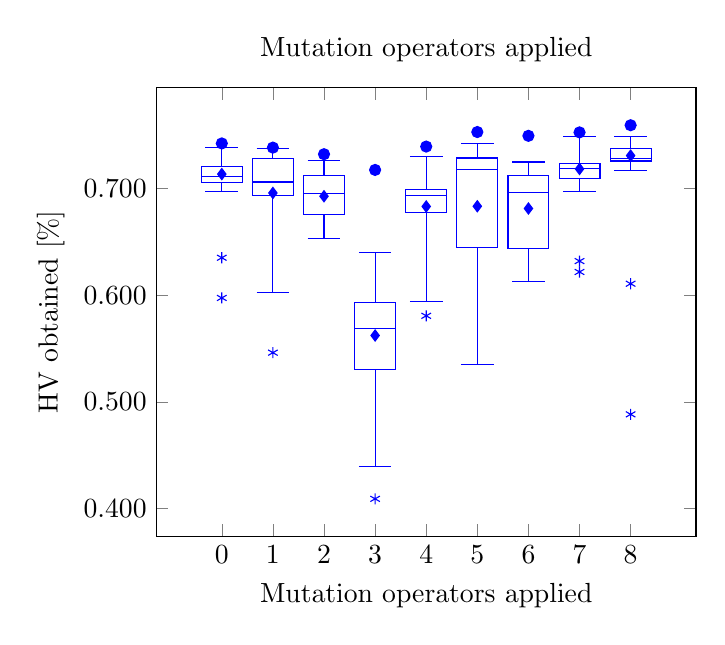
\begin{tikzpicture} 
\begin{axis}[ 
title={Mutation operators applied}, 
boxplot/draw direction=y, 
xtick={1,2,3,4,5,6,7,8,9}, 
xticklabels={0,1,2,3,4,5,6,7,8}, 
x tick label style={rotate=0, align=center}, 
xlabel={Mutation operators applied}, 
y tick label style={/pgf/number format/.cd,fixed,precision=3, zerofill}, 
ylabel={HV obtained [\%]}, 
] 

% ############## Mutations_AMALGAM=0 ################## 
\addplot[boxplot, mark=asterisk, 
boxplot prepared={ 
lower whisker=0.69746, 
upper whisker=0.73837, 
lower quartile=0.7058, 
upper quartile=0.72069, 
median=0.71142, 
average=0.71374}, 
color = blue, solid, area legend] 
coordinates {
(1,0.63529)
(1,0.59759)}; 
\addplot[only marks,mark=*,color = blue]coordinates{(1,0.74249)}; 

% ############## Mutations_AMALGAM=1 ################## 
\addplot[boxplot, mark=asterisk, 
boxplot prepared={ 
lower whisker=0.60266, 
upper whisker=0.73809, 
lower quartile=0.69349, 
upper quartile=0.72866, 
median=0.70628, 
average=0.69607}, 
color = blue, solid, area legend] 
coordinates {
(2,0.54628)}; 
\addplot[only marks,mark=*,color = blue]coordinates{(2,0.73858)}; 

% ############## Mutations_AMALGAM=2 ################## 
\addplot[boxplot, mark=asterisk, 
boxplot prepared={ 
lower whisker=0.65317, 
upper whisker=0.72623, 
lower quartile=0.67623, 
upper quartile=0.71254, 
median=0.69516, 
average=0.69299}, 
color = blue, solid, area legend] 
coordinates {}; 
\addplot[only marks,mark=*,color = blue]coordinates{(3,0.73241)}; 

% ############## Mutations_AMALGAM=3 ################## 
\addplot[boxplot, mark=asterisk, 
boxplot prepared={ 
lower whisker=0.43986, 
upper whisker=0.6406, 
lower quartile=0.53017, 
upper quartile=0.59331, 
median=0.56928, 
average=0.56239}, 
color = blue, solid, area legend] 
coordinates {
(4,0.40921)}; 
\addplot[only marks,mark=*,color = blue]coordinates{(4,0.71764)}; 

% ############## Mutations_AMALGAM=4 ################## 
\addplot[boxplot, mark=asterisk, 
boxplot prepared={ 
lower whisker=0.59418, 
upper whisker=0.72999, 
lower quartile=0.67745, 
upper quartile=0.69944, 
median=0.69363, 
average=0.6834}, 
color = blue, solid, area legend] 
coordinates {
(5,0.58085)}; 
\addplot[only marks,mark=*,color = blue]coordinates{(5,0.73956)}; 

% ############## Mutations_AMALGAM=5 ################## 
\addplot[boxplot, mark=asterisk, 
boxplot prepared={ 
lower whisker=0.53483, 
upper whisker=0.74254, 
lower quartile=0.64475, 
upper quartile=0.72887, 
median=0.71785, 
average=0.68359}, 
color = blue, solid, area legend] 
coordinates {}; 
\addplot[only marks,mark=*,color = blue]coordinates{(6,0.75319)}; 

% ############## Mutations_AMALGAM=6 ################## 
\addplot[boxplot, mark=asterisk, 
boxplot prepared={ 
lower whisker=0.61292, 
upper whisker=0.72511, 
lower quartile=0.64405, 
upper quartile=0.71264, 
median=0.6963, 
average=0.68149}, 
color = blue, solid, area legend] 
coordinates {}; 
\addplot[only marks,mark=*,color = blue]coordinates{(7,0.74963)}; 

% ############## Mutations_AMALGAM=7 ################## 
\addplot[boxplot, mark=asterisk, 
boxplot prepared={ 
lower whisker=0.69714, 
upper whisker=0.74889, 
lower quartile=0.70972, 
upper quartile=0.72389, 
median=0.71871, 
average=0.71859}, 
color = blue, solid, area legend] 
coordinates {
(8,0.62196)
(8,0.63217)}; 
\addplot[only marks,mark=*,color = blue]coordinates{(8,0.75286)}; 

% ############## Mutations_AMALGAM=8 ################## 
\addplot[boxplot, mark=asterisk, 
boxplot prepared={ 
lower whisker=0.71749, 
upper whisker=0.74937, 
lower quartile=0.72603, 
upper quartile=0.73795, 
median=0.7284, 
average=0.73109}, 
color = blue, solid, area legend] 
coordinates {
(9,0.61093)
(9,0.48844)}; 
\addplot[only marks,mark=*,color = blue]coordinates{(9,0.75956)}; 

\end{axis}
\end{tikzpicture}
\end{figure} 

% ######################## UTRP SA Mutation operators applied ######################## 
\begin{figure} 
\centering 
\tikzsetnextfilename{UTRP_DBMOSA_BP_mutation_funcs_AMAL_every_n} 
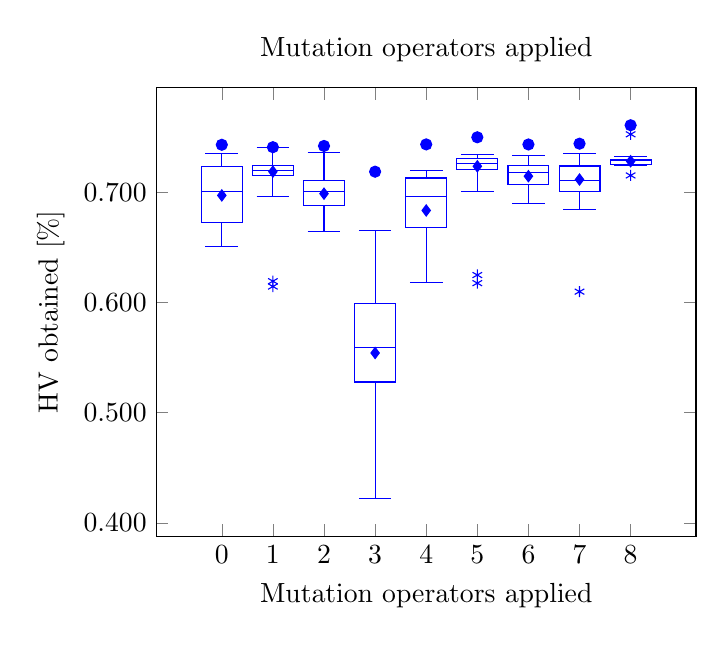
\begin{tikzpicture} 
\begin{axis}[ 
title={Mutation operators applied}, 
boxplot/draw direction=y, 
xtick={1,2,3,4,5,6,7,8,9}, 
xticklabels={0,1,2,3,4,5,6,7,8}, 
x tick label style={rotate=0, align=center}, 
xlabel={Mutation operators applied}, 
y tick label style={/pgf/number format/.cd,fixed,precision=3, zerofill}, 
ylabel={HV obtained [\%]}, 
] 

% ############## Mutations_AMALGAM_every_n=0 ################## 
\addplot[boxplot, mark=asterisk, 
boxplot prepared={ 
lower whisker=0.65079, 
upper whisker=0.7355, 
lower quartile=0.6727, 
upper quartile=0.72346, 
median=0.70056, 
average=0.69724}, 
color = blue, solid, area legend] 
coordinates {}; 
\addplot[only marks,mark=*,color = blue]coordinates{(1,0.74318)}; 

% ############## Mutations_AMALGAM_every_n=1 ################## 
\addplot[boxplot, mark=asterisk, 
boxplot prepared={ 
lower whisker=0.69585, 
upper whisker=0.74043, 
lower quartile=0.71491, 
upper quartile=0.72442, 
median=0.71959, 
average=0.71879}, 
color = blue, solid, area legend] 
coordinates {
(2,0.6194)
(2,0.61457)}; 
\addplot[only marks,mark=*,color = blue]coordinates{(2,0.741)}; 

% ############## Mutations_AMALGAM_every_n=2 ################## 
\addplot[boxplot, mark=asterisk, 
boxplot prepared={ 
lower whisker=0.66422, 
upper whisker=0.73657, 
lower quartile=0.68832, 
upper quartile=0.71071, 
median=0.70092, 
average=0.6988}, 
color = blue, solid, area legend] 
coordinates {}; 
\addplot[only marks,mark=*,color = blue]coordinates{(3,0.74212)}; 

% ############## Mutations_AMALGAM_every_n=3 ################## 
\addplot[boxplot, mark=asterisk, 
boxplot prepared={ 
lower whisker=0.42191, 
upper whisker=0.66521, 
lower quartile=0.52795, 
upper quartile=0.59944, 
median=0.55902, 
average=0.55424}, 
color = blue, solid, area legend] 
coordinates {}; 
\addplot[only marks,mark=*,color = blue]coordinates{(4,0.71877)}; 

% ############## Mutations_AMALGAM_every_n=4 ################## 
\addplot[boxplot, mark=asterisk, 
boxplot prepared={ 
lower whisker=0.61787, 
upper whisker=0.71988, 
lower quartile=0.66778, 
upper quartile=0.713, 
median=0.69622, 
average=0.68362}, 
color = blue, solid, area legend] 
coordinates {}; 
\addplot[only marks,mark=*,color = blue]coordinates{(5,0.74353)}; 

% ############## Mutations_AMALGAM_every_n=5 ################## 
\addplot[boxplot, mark=asterisk, 
boxplot prepared={ 
lower whisker=0.7005, 
upper whisker=0.73416, 
lower quartile=0.72081, 
upper quartile=0.73074, 
median=0.72638, 
average=0.72367}, 
color = blue, solid, area legend] 
coordinates {
(6,0.62499)
(6,0.61763)}; 
\addplot[only marks,mark=*,color = blue]coordinates{(6,0.74998)}; 

% ############## Mutations_AMALGAM_every_n=6 ################## 
\addplot[boxplot, mark=asterisk, 
boxplot prepared={ 
lower whisker=0.6896, 
upper whisker=0.7335, 
lower quartile=0.70686, 
upper quartile=0.72404, 
median=0.71778, 
average=0.71467}, 
color = blue, solid, area legend] 
coordinates {}; 
\addplot[only marks,mark=*,color = blue]coordinates{(7,0.74347)}; 

% ############## Mutations_AMALGAM_every_n=7 ################## 
\addplot[boxplot, mark=asterisk, 
boxplot prepared={ 
lower whisker=0.68432, 
upper whisker=0.73509, 
lower quartile=0.70112, 
upper quartile=0.72395, 
median=0.71066, 
average=0.71164}, 
color = blue, solid, area legend] 
coordinates {
(8,0.6099)}; 
\addplot[only marks,mark=*,color = blue]coordinates{(8,0.74418)}; 

% ############## Mutations_AMALGAM_every_n=8 ################## 
\addplot[boxplot, mark=asterisk, 
boxplot prepared={ 
lower whisker=0.72415, 
upper whisker=0.73277, 
lower quartile=0.7256, 
upper quartile=0.72993, 
median=0.72857, 
average=0.72825}, 
color = blue, solid, area legend] 
coordinates {
(9,0.71536)
(9,0.75269)}; 
\addplot[only marks,mark=*,color = blue]coordinates{(9,0.76092)}; 

\end{axis}
\end{tikzpicture}
\end{figure} 

% ######################## UTRP SA Mutation operators applied ######################## 
\begin{figure} 
\centering 
\tikzsetnextfilename{UTRP_DBMOSA_BP_mutation_funcs_Counts_normal} 
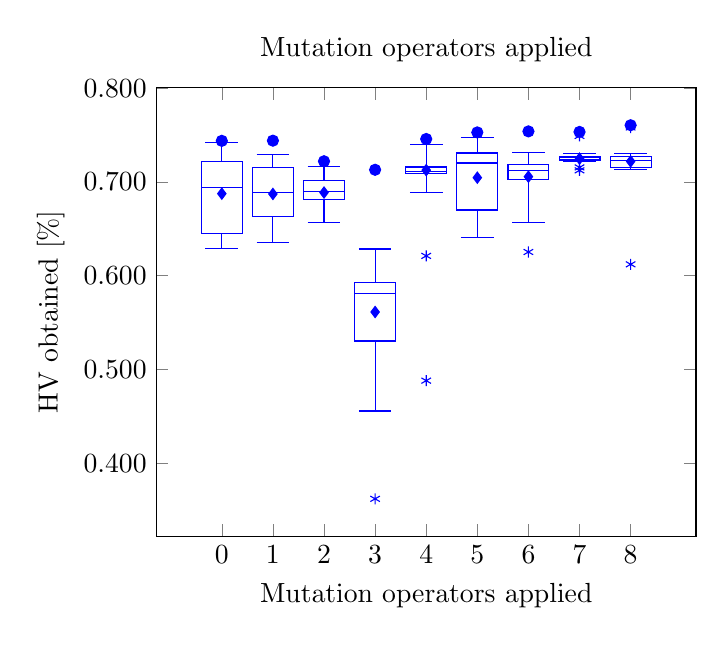
\begin{tikzpicture} 
\begin{axis}[ 
title={Mutation operators applied}, 
boxplot/draw direction=y, 
xtick={1,2,3,4,5,6,7,8,9}, 
xticklabels={0,1,2,3,4,5,6,7,8}, 
x tick label style={rotate=0, align=center}, 
xlabel={Mutation operators applied}, 
y tick label style={/pgf/number format/.cd,fixed,precision=3, zerofill}, 
ylabel={HV obtained [\%]}, 
] 

% ############## Mutations_Counts_normal=0 ################## 
\addplot[boxplot, mark=asterisk, 
boxplot prepared={ 
lower whisker=0.62882, 
upper whisker=0.74202, 
lower quartile=0.64502, 
upper quartile=0.72197, 
median=0.69403, 
average=0.68749}, 
color = blue, solid, area legend] 
coordinates {}; 
\addplot[only marks,mark=*,color = blue]coordinates{(1,0.74386)}; 

% ############## Mutations_Counts_normal=1 ################## 
\addplot[boxplot, mark=asterisk, 
boxplot prepared={ 
lower whisker=0.63549, 
upper whisker=0.7293, 
lower quartile=0.66286, 
upper quartile=0.71573, 
median=0.68873, 
average=0.68719}, 
color = blue, solid, area legend] 
coordinates {}; 
\addplot[only marks,mark=*,color = blue]coordinates{(2,0.74405)}; 

% ############## Mutations_Counts_normal=2 ################## 
\addplot[boxplot, mark=asterisk, 
boxplot prepared={ 
lower whisker=0.65668, 
upper whisker=0.71695, 
lower quartile=0.6811, 
upper quartile=0.70174, 
median=0.69016, 
average=0.6887}, 
color = blue, solid, area legend] 
coordinates {}; 
\addplot[only marks,mark=*,color = blue]coordinates{(3,0.72208)}; 

% ############## Mutations_Counts_normal=3 ################## 
\addplot[boxplot, mark=asterisk, 
boxplot prepared={ 
lower whisker=0.45566, 
upper whisker=0.62843, 
lower quartile=0.53028, 
upper quartile=0.59295, 
median=0.58131, 
average=0.56124}, 
color = blue, solid, area legend] 
coordinates {
(4,0.36192)}; 
\addplot[only marks,mark=*,color = blue]coordinates{(4,0.71298)}; 

% ############## Mutations_Counts_normal=4 ################## 
\addplot[boxplot, mark=asterisk, 
boxplot prepared={ 
lower whisker=0.68866, 
upper whisker=0.73995, 
lower quartile=0.70876, 
upper quartile=0.71597, 
median=0.7108, 
average=0.71258}, 
color = blue, solid, area legend] 
coordinates {
(5,0.488)
(5,0.62112)}; 
\addplot[only marks,mark=*,color = blue]coordinates{(5,0.74583)}; 

% ############## Mutations_Counts_normal=5 ################## 
\addplot[boxplot, mark=asterisk, 
boxplot prepared={ 
lower whisker=0.64038, 
upper whisker=0.74705, 
lower quartile=0.67004, 
upper quartile=0.73087, 
median=0.72026, 
average=0.7046}, 
color = blue, solid, area legend] 
coordinates {}; 
\addplot[only marks,mark=*,color = blue]coordinates{(6,0.75287)}; 

% ############## Mutations_Counts_normal=6 ################## 
\addplot[boxplot, mark=asterisk, 
boxplot prepared={ 
lower whisker=0.65648, 
upper whisker=0.73141, 
lower quartile=0.70299, 
upper quartile=0.71905, 
median=0.7118, 
average=0.70564}, 
color = blue, solid, area legend] 
coordinates {
(7,0.62527)}; 
\addplot[only marks,mark=*,color = blue]coordinates{(7,0.75395)}; 

% ############## Mutations_Counts_normal=7 ################## 
\addplot[boxplot, mark=asterisk, 
boxplot prepared={ 
lower whisker=0.72211, 
upper whisker=0.72988, 
lower quartile=0.72283, 
upper quartile=0.72662, 
median=0.7235, 
average=0.72491}, 
color = blue, solid, area legend] 
coordinates {
(8,0.7155)
(8,0.71238)
(8,0.74907)}; 
\addplot[only marks,mark=*,color = blue]coordinates{(8,0.75339)}; 

% ############## Mutations_Counts_normal=8 ################## 
\addplot[boxplot, mark=asterisk, 
boxplot prepared={ 
lower whisker=0.71329, 
upper whisker=0.73034, 
lower quartile=0.71544, 
upper quartile=0.7269, 
median=0.72309, 
average=0.72196}, 
color = blue, solid, area legend] 
coordinates {
(9,0.75812)
(9,0.6121)}; 
\addplot[only marks,mark=*,color = blue]coordinates{(9,0.76051)}; 

\end{axis}
\end{tikzpicture}
\end{figure} 
\begin{table}
\centering
\caption{Legend for the boxplot.}
\begin{tabular}{ll}
\toprule
 Index &                                               Name \\
\midrule
     0 &               [MSC\_add\_terminal, MSC\_del\_terminal] \\
     1 &                        [Add\_vertex, Delete\_vertex] \\
     2 &       [Trim\_one\_terminal\_cb, Grow\_one\_terminal\_cb] \\
     3 &       [Insert\_inside\_vertex, Delete\_inside\_vertex] \\
     4 & [Add\_vertex, Delete\_vertex, Insert\_inside\_verte... \\
     5 &        [Add\_vertex, Delete\_vertex, Intertwine\_two] \\
     6 & [Add\_vertex, Delete\_vertex, Insert\_inside\_verte... \\
     7 & [MSC\_add\_terminal, MSC\_del\_terminal, Insert\_ins... \\
     8 & [Add\_vertex, Delete\_vertex, Insert\_inside\_verte... \\
\bottomrule
\end{tabular}
\end{table}

\end{document}
